%%%%%%%%%%%%%%%%%%%%%%
%%%%%%%%%%%%%%%%%%%%%%
%
%                                        PRE-AMBLE
%
%%%%%%%%%%%%%%%%%%%%%%
%%%%%%%%%%%%%%%%%%%%%%

\documentclass[11pt]{amsart}

\setlength{\textwidth}{\paperwidth}
\addtolength{\textwidth}{-3in}
\calclayout

% LOAD PACKAGES--------------------------------------------

\usepackage{amsfonts, amsthm, amssymb, amsmath, stmaryrd, etoolbox}
\usepackage{comment}
\usepackage{mathtools}
\usepackage{graphicx,caption,subcaption}
\usepackage{todonotes}
\usepackage{xcolor}

\usepackage[inline]{enumitem}
\setlist{itemsep=0em, topsep=0em, parsep=0em}
\setlist[enumerate]{label=(\alph*)}

\usepackage{tikz}
\usepackage[all,2cell]{xy}
\usetikzlibrary{matrix,arrows,shapes,decorations.markings,decorations.pathreplacing}
\definecolor{rewritecolor}{rgb}{0,.9,1}
\tikzset{rewritenode/.style={shape=circle,fill=rewritecolor,scale=0.25,font=\Huge}}
\tikzset{RWopen/.style={shape=circle,draw=black,fill=white,scale=0.5,font=\Huge}}
\tikzset{RWclosed/.style={shape=circle,fill=black,scale=0.5,font=\Huge}}
\tikzset{CDnode/.style={shape=circle,fill=white,scale=.5}}
\tikzset{zxgreen/.style={shape=circle,draw,thick,fill=green}}
\tikzset{zxred/.style={shape=circle,draw,thick,fill=red}}
\tikzset{zxyellow/.style={shape=rectangle,draw,thick,fill=yellow}}
\tikzset{zxdiamond/.style={shape=diamond,fill=black,inner sep=2.75}}
\tikzset{zxopen/.style={shape=circle,draw,thick,inner sep=2pt}}
\tikzset{->-/.style={decoration={%
			markings,
			mark=at position .5 with {\arrow{>}}},postaction={decorate}}
}
\tikzset{->-pos/.style={decoration={%
			markings,
			mark=at position #1 with {\arrow{>}}},postaction={decorate}}
}

\usepackage{hyperref}
\definecolor{hyperrefcolor}{rgb}{0,0,0.7}
\hypersetup{colorlinks,linkcolor={hyperrefcolor},citecolor={hyperrefcolor},urlcolor={hyperrefcolor}}

%NEW COMMANDS---------------------------------------------

\newcommand{\cl}[1]{\mathcal{#1}}
\newcommand{\scr}[1]{\mathscr{#1}}
\newcommand{\op}[1]{\operatorname{#1}}
\newcommand{\cat}[1]{\mathbf{#1}}
\newcommand{\dblcat}[1]{\mathbb{#1}}
\renewcommand{\t}[1]{\textup{#1}}

\newcommand{\from}{\colon}
\newcommand{\xto}[1]{\xrightarrow{#1}}
\newcommand{\sm}{\smallsetminus}
\newcommand{\tospan}{\xrightarrow{\mathit{sp}}}
\newcommand{\tocospan}{\xrightarrow{\mathit{csp}}}

%\newcommand{\diagram}[1]{\raisebox{-0.5\height}{\includegraphics{#1}}}

\newcommand{\bluebullet}{\textcolor{rewritecolor}{\bullet}}

%  macros for (co)span bicategories
\newcommand{\bispmap}[1]{\mathbf{Sp(#1)}}
\newcommand{\dblspmap}[1]{\mathbb{S}\mathbf{p(#1)}}
\newcommand{\bicspmap}[1]{\mathbf{Csp(#1)}}
\newcommand{\dblcspmap}[1]{\mathbb{C}\mathbf{sp(#1)}}
\newcommand{\bispsp}[1]{\mathbf{Sp(Sp(#1))}}
\newcommand{\dblspsp}[1]{\mathbb{S}\mathbf{p(Sp(#1))}}
\newcommand{\bicspcsp}[1]{\mathbf{Csp(Csp(#1))}}
\newcommand{\dblcspcsp}[1]{\mathbb{C}\mathbf{sp(Csp(#1))}}
\newcommand{\bimonspcsp}[1]{\mathbf{MonicSp(Csp(#1))}}
\newcommand{\dblmonspcsp}[1]{\mathbb{M}\mathbf{onicSp(Csp(#1))}}
\newcommand{\biepiccspsp}[1]{\mathbf{EpicCsp(Sp(#1))}}
\newcommand{\dblepiccspsp}[1]{\mathbb{E}\mathbf{picCsp(Sp(#1))}}
\newcommand{\bispcs}[1]{\mathbf{Sp}(\mathbf{Csp}(\mathbf{#1}))}

% defining arrow with a vertical line through it
\makeatletter
\def\slashedarrowfill@#1#2#3#4#5{%
	$\m@th\thickmuskip0mu\medmuskip\thickmuskip\thinmuskip\thickmuskip
	\relax#5#1\mkern-7mu%
	\cleaders\hbox{$#5\mkern-2mu#2\mkern-2mu$}\hfill
	\mathclap{#3}\mathclap{#2}%
	\cleaders\hbox{$#5\mkern-2mu#2\mkern-2mu$}\hfill
	\mkern-7mu#4$%
}
\def\rightslashedarrowfill@{%
	\slashedarrowfill@\relbar\relbar\mapstochar\rightarrow}
\newcommand{\xslashedrightarrow}[2][]{%
	\ext@arrow 0055{\rightslashedarrowfill@}{#1}{#2}}
\makeatother

\newcommand{\hto}{\xslashedrightarrow{}}


%DECLARE MATH OPERATORS----------------------------------

\DeclareMathOperator{\Hom}{Hom}
\DeclareMathOperator{\id}{id}
\DeclareMathOperator{\ob}{Ob}
\DeclareMathOperator{\arr}{arr}
\DeclareMathOperator{\im}{im}
\DeclareMathOperator{\Aut}{Aut}
\DeclareMathOperator{\Bij}{Bij}
\DeclareMathOperator{\Sub}{Sub}
\DeclareMathOperator{\decat}{decat}

%ENVIRONMENTS AND COUNTERS---------------------------------

\newtheorem{thm}{Theorem}[section]
\newtheorem{lem}[thm]{Lemma}
\newtheorem{prop}[thm]{Proposition}
\newtheorem{cor}[thm]{Corollary}

\theoremstyle{remark}
\newtheorem{remark}[thm]{Remark}
\newtheorem{notation}[thm]{Notation}

\theoremstyle{definition}
\newtheorem{ex}[thm]{Example} 
\newtheorem{defn}[thm]{Definition}

%\setcounter{tocdepth}{1} % Sets depth for table of contents. 

% FOR THIS PAPER ONLY

\newcommand{\zx}{_{\text{zx}}}
\newcommand{\bicat}[1]{\underline{\mathbf{#1}}}
\newcommand{\SpCspZX}{\cat{Sp}(\cat{Csp}(\cat{Graph}\downarrow S_{\text{zx}}))}
\newcommand{\zxGraphs}{\cat{Graph} \downarrow S_{\text{zx}}}

%%%%%%%%%%%%%%%%%%%%%%
%%%%%%%%%%%%%%%%%%%%%%
%%%%%%%%%%%%%%%%%%%%%%
%%%%%%%%%%%%%%%%%%%%%%
%
%BEGIN DOCUMENT
%
%%%%%%%%%%%%%%%%%%%%%%
%%%%%%%%%%%%%%%%%%%%%%
%%%%%%%%%%%%%%%%%%%%%%
%%%%%%%%%%%%%%%%%%%%%%

\begin{document}
	
%\tableofcontents

\begin{abstract}
	This paper presents a symmetric monoidal and compact closed bicategory that categorifies the zx-calculus developed by Coecke and Duncan.  The $1$-cells in this bicategory are certain graph morphisms that correspond to the string diagrams of the zx-calculus, while the $2$-cells are rewrite rules. 
\end{abstract}

\title{Categorifying the zx-calculus}
\author{Daniel Cicala}
\maketitle

%%%%%%%%%%%%%%%%%%%%%%
%%%%%%%%%%%%%%%%%%%%%%
% INTRODUCTION
\section{Introduction}
\label{sec:Introduction}
%%%%%%%%%%%%%%%%%%%%%%
%%%%%%%%%%%%%%%%%%%%%%

Compositionality is becoming increasingly recognized as a viable method to model complex systems such as those found in physics \cite{AbramCoecke_CatSemanticQuantum}, computer science \cite{SassoneSobocinski_PetriNets}, and biology \cite{BaezFongPollard_CompMarkovProcesses}.  The idea is to study smaller, simpler systems and ways of connecting them together.  The word \emph{compositionality} suggests that category theory can play a key role, and indeed it does.  Systems are morphisms and connections are morphism composition.   

This paper looks at one example of compositionality in action: the zx-calculus.  The backstory dates to Penrose's tensor networks \cite{Penrose_NegDimTensors} and, more recently, to the relationship between graphical languages and monoidal categories explored by Joyal, Street, and Selinger \cite{JoyalStreet_GeomTensorCalc,Selinger_GraphicsMonCats}.  Abramsky and Coecke capitalized on this relationship when inventing a categorical framework for quantum physics \cite{AbramCoecke_CatSemanticQuantum}.  With a categorically oriented point of view, Coecke and Duncan  presented early results on a diagrammatic language in which to reason about complementary quantum observables \cite{CoeckeDuncan_QuantumObsInitialReport}. After a fruitful period of development \cite{CoeckeEdwards_ToyTheories,CoeckeEdwardsSpekkens_PhaseGrpsNonLocality,CoeckePerdix_EnvironClassicChannels,DuncanPerdix_GraphStatesEulerDecomp,DuncanPerdrix_RewritingQuantumCompu,EvansDuncanLangPanan_ClassMutualUnbias,Pavlovic_QuanClassNondetermCompu}, the first complete presentation of the zx-calculus was published \cite{CoeckeDuncan_QuantumObsFullPaper}.  

The zx-calculus contains five basic diagrams, depicted in Figure \ref{fig:ZX generators}.
\begin{figure}
	\fbox{%
		\begin{minipage}{\textwidth}
			\centering
			%%%%%%%%%%%%%%%%%%%%%%
			\subcaptionbox{Wire}[.1\textwidth]{%
				
\includegraphics{generater_wire}
			}
			~
			\subcaptionbox{Green spider}[.2\textwidth]{%
				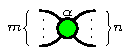
\includegraphics{generater_green_spider}
			}
			~
			\subcaptionbox{Red spider}[.2\textwidth]{%
				
\includegraphics{generater_red_spider}
			}
			~
			\subcaptionbox{Hadamard}[.2\textwidth]{%
				
\includegraphics[]{generater_hadamard}
			}
			~
			\subcaptionbox{Diamond}[.15\textwidth]{%
				
\includegraphics{generater_diamond}
			}
			%%%%%%%%%%%%%%%%%%%%%%
		\end{minipage}
	}
	\caption{Generators for the category $\cat{zx}$}
	\label{fig:ZX generators}
\end{figure}
These can be combined in various ways to form larger, more complex diagrams.   Observe that these diagrams have dangling wires on the left and right. Think of those on the left as inputs and those on the right as outputs.  Formalizing this perspective, we let these diagrams generate the morphisms of a dagger compact category $\cat{zx}$ whose objects are the non-negative integers, the meaning of which is number of inputs and outputs.  Section \ref{sec:ZxCalc} contains a formal introduction to the zx-calculus.  This is a merely a brief primer and contains nothing new.  There, we also touch on various software tools, such as Quantomatic \cite{BarKissingerVicary_Globular,DixonDuncanKissinger_QuantomaticWebsite} or Globular \cite{BarKissingerVicary_Globular}, used to compute with the types of diagrams found in the zx-calculus.  

Our goal in this paper is to introduce a symmetric monoidal and compact closed (SMCC) bicategory $\bicat{zx}$ that categorifies $\cat{zx}$ in the sense that the $1$-cells of $\bicat{zx}$ will correspond to the zx-diagrams.  Building this correspondence, however, requires a bit of labor. We begin Section \ref{sec:RewritingOpenGraphs} by discussing open graphs and starting construction on a bicategory that suitably houses these open graphs.  With this in mind, we slightly modify past work of the author and Courser \cite{Cicala_SpansCospans, CicalaCourser_BicatSpansCospan} to produce an SMCC-bicategory with graphs as $0$-cells, cospans of graphs as $1$-cells, and certain isomorphism classes of spans of cospans (see Figure \ref{fig:spans of cospans}) of graphs as $2$-cells.   
\begin{figure}
	\fbox{%
		\begin{minipage}{\textwidth}
			\centering
			\subcaptionbox{A span of cospans}[.4\textwidth]{%
				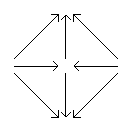
\includegraphics{diagram_span_cospans}
			}
			~
			\subcaptionbox{A span of cospans morphism}[.4\textwidth]{%
				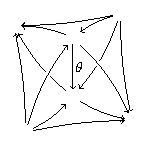
\includegraphics{(scC)+(Map_of_Spans_of_Cospans)}
			}
		\end{minipage}
	}
	\caption{A generic $2$-cell in $\bispcs{C}$}
	\label{fig:spans of cospans}
\end{figure}
This has a $1$-full and $2$-full sub-bicategory $\cat{Rewrite}$ consisting of non-negative integers as $0$-cells, open graphs as $1$-cells, and rewrite rules of open graphs as $2$-cells.  The SMCC bicategory $\cat{Rewrite}$ is a nice ambient space in which to generate systems modeled on open graphs.  In this paper, we exploit $\cat{Rewrite}$ to model the zx-calculus.

In Section \ref{sec:OpenGraphsOverSzx}, we discuss \emph{open graphs over $S\zx$}.  That is, we pick a graph $S\zx$
\[
	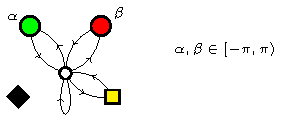
\includegraphics{graph_S_zx}
\]  
in such a way that graph morphisms $G \to S\zx$ correspond exactly to the zx-morphisms.  These form an SMCC bicategory with graphs over $S\zx$ as $0$-cells, cospans of graphs over $S\zx$ as $1$-cells, and certain isomorphism classes of spans of these cospans as $2$-cells.  This contains a sub-bicategory named $\cat{zxRewrite}$ that is analogous to $\cat{Rewrite}$, if not as immediate.  Indeed, to define this, we first introduce the functor $N\zx \from \cat{Set}_0 \to \left( \zxGraphs \right)$ on a skeleton of the category $\cat{Set}$.  Define $N\zx(X)$ to be the edgeless graph with nodes $X$ and is constant on the $S\zx$-node $
\begin{tikzpicture} \node [zxopen] at (0,0) {}; \end{tikzpicture}$.  Then $\cat{zxRewrite}$ is $1$-full and $2$-full on the $0$-cells of form $N\zx (X)$.  

Now, $\cat{zxRewrite}$ is a space in which we can generate SMCC sub-bicategories. In Section \ref{sec:zx categorified}, we give a presentation for a sub-bicategory $\bicat{zx}$ of $\cat{zxRewrite}$ by choosing $1$-cell corresponding to diagrams of the zx-calculus and $2$-cells corresponding to relations that hold between diagrams.  After constructing $\bicat{zx}$, we decategorify it to a $1$-category $\decat(\bicat{zx})$ by identifying $1$-cells whenever there is a $2$-cell between them.  Though this seems asymmetrical, the dual nature of spans allows this to actually give an equivalence relation, not merely generate one.  Our main result is Theorem \ref{thm:equiv of zx cats}, in which we construct a dagger compact functor $\decat(\bicat{zx}) \to \cat{zx}$ that is an equivalence of categories.  

The author would like to thank his advisor John Baez for many helpful ideas and discussions that contributed to this paper.   

%%%%%%%%%%%%%%%%%%%%%%
%%%%%%%%%%%%%%%%%%%%%%
% THE ZX-CALCULUS
\section{The zx-calculus}
\label{sec:ZxCalc}
%%%%%%%%%%%%%%%%%%%%%%
%%%%%%%%%%%%%%%%%%%%%%

One of the most fascinating features of quantum physics is the incompatibility of observables. Roughly, an observable is a measurable quantity of some system, for instance the spin of a photon.  Incompatibility is in stark contrast to classical physics in which measurable quantities are compatible, in that they can have arbitrarily precise values at the same time.   Arguably, the most famous example of incompatibility is Heisenberg's uncertainty principal which places limits to the precision that one can simultaneously measure a pair of observables: position and momentum.  There are different levels of incompatibility amongst pairs of observables. When such a pair is maximally incompatible, in the sense that knowing one with complete precision implies total uncertainty of the other, we say they are \emph{complementary observables}.  

Historically, the typical framework in which one might study observables is Hilbert space.  In a Hilbert space, each vector represents the state of a given system. Even though this formalism has been incredibly fruitful, computations in Hilbert spaces can be difficult and non-intuitive. The zx-calculus was developed by Coecke and Duncan \cite{CoeckeDuncan_QuantumObsFullPaper} as a high-level language to facilitate such computation.  It was immediately used to generalize both \emph{quantum circuits} \cite{NielsenChuang_QuantumCompInfo}  and the \emph{measurement calculus} \cite{DanosKashefiPanang_MeasurementCalc}. Its validity was further justified when Duncan and Perdrix presented a non-trivial method of verifying measurement-based quantum computations with the zx-calculus \cite{DuncanPerdrix_RewritingQuantumCompu}.  At its core, the zx-calculus is an intuitive graphical language in which to reason about complementary observables. 

The five \emph{basic diagrams} in the zx-calculus are depicted in Figure \ref{fig:ZX generators} and are to be read from left to right. They are
\begin{itemize}
	\item a \emph{wire} with a single input and output,
	\item \emph{green spiders} with a non-negative integer number of inputs and outputs and paired with a phase $\alpha \in [-\pi,\pi)$,
	\item \emph{red spiders} with a non-negative integer number inputs and outputs and paired with a phase $\beta \in [-\pi,\pi)$,
	\item the \emph{Hadamard node} with a single input and output, and
	\item a \emph{black diamond node} with no inputs or outputs.
\end{itemize}
The wire plays the role of an identity, much like a plain wire in an electrical circuit, or straight pipe in a plumbing system. The green and red spiders arise from a pair of complementary observables.  Incredibly, observables correspond to certain commutative Frobenius algebras $A$ living in a dagger symmetric monoidal category $\cat{C}$. Moreover, a pair of complementary observables gives a pair of Frobenius algebras whose operations interact via laws like those of a Hopf algebra \cite{CoeckePavlovic_QuantumMeasSums, CoeckePavVicary_OrthBasis}.  This is particularly nice because Frobenius algebras have beautiful representations as string diagrams. Hence the depiction of the spiders. Now, if $I$ is the monoidal unit of $\cat{C}$, there is an isomorphism $\cat{C}(I,A) \to \cat{C}(A,A)$ of commutative monoids that gives rise to a group on $A$ known as the \emph{phase group}.  It is from this that we get the phases on the spiders. The Hadamard node embodies the Hadamard gate. The diamond follows from the notion of \emph{coherence}, which exists between observable structures if certain equations are satisfied.  A deeper exploration of these notions goes beyond the scope of this paper.  For interested readers, there are already excellent treatments of these topics \cite{CoeckeDuncan_QuantumObsFullPaper}.

In the spirit of compositionality, we will present a category $\cat{zx}$ whose morphisms are generated by the five diagrams in Figure \ref{fig:ZX generators}. Therefore, we will go ahead and call the basic diagrams in Figure \ref{fig:ZX generators} \emph{basic $\cat{zx}$-morphisms} and call a diagram an \emph{$\cat{zx}$-morphism} if it is generated by a basic one.

Observe that, on the basic $\cat{zx}$-morphisms, there is a non-negative number of dangling wires on the right and left sides. We will refer to the wires on the left as \emph{inputs} and those on the right as \emph{outputs}. With this in mind, we now present the dagger compact category $\cat{zx}$ introduced by Coecke and Duncan \cite{CoeckeDuncan_QuantumObsFullPaper} and further studied by Backens \cite{Backens_Completeness}. The objects of $\cat{zx}$ are the non-negative integers.  The morphisms are generated by the basic $\cat{zx}$-morphisms, though we take the wire to be the identity on $1$.  Composition in $\cat{zx}$ is performed by separately enumerating the inputs and outputs of a pair of compatible diagrams  and connecting the outputs of the first diagram to the inputs of the second diagram accordingly.  The monoidal product on $\cat{zx}$ is given by addition of numbers and the disjoint union of $\cat{zx}$-morphisms. From this, we obtain the identity on any $n$ by taking the disjoint union of $n$ wires. The symmetry and compactness of the monoidal product provide a braiding, evaluation, and coevaluation morphisms, respectively,
\[

\includegraphics{morphism_zx_braiding}
\quad \quad \quad \quad 
\raisebox{-0.25\height}{%
	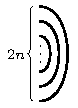
\includegraphics[scale=0.75]{morphism_zx_evaluation}
}
\quad \quad \quad \quad 
\raisebox{-0.25\height}{%
	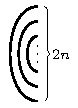
\includegraphics[scale=0.75]{morphism_zx_coevaluation}
}
\]
The evaluation and coevalutation maps are of type $2n \to 0$ and $0 \to 2n$ for each object $n \geq 1$ and the empty diagram for $n=0$.  The dagger structure is obtained by swapping inputs and outputs then, for the spider diagrams, multiplying the phase by $-1$.  For instance, 
\[
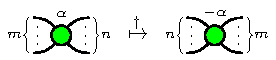
\includegraphics{functor_dagger}
\]
The dagger acts trivially on the wire, Hadamard, and diamond elements. 

\begin{figure}[h]
	\fbox{
		\begin{minipage}{\textwidth}
			\centering
			%%%%%%%%%%%%%%%%%%%%%%
			\begin{subfigure}[t]{0.4\textwidth}
				\centering
				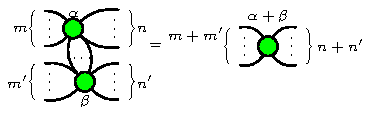
\includegraphics{equation_spider}
				\caption{Spider equation}
			\end{subfigure}%
			~
			\begin{subfigure}[t]{0.5\textwidth}
				\centering
				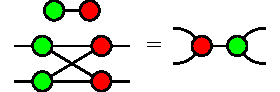
\includegraphics{equation_bialgebra}
				\caption{Bialgebra equation}
			\end{subfigure}%
			%%%%%%%%%%%%%%%%%%%%%%
			\vspace{2ex}
			%%%%%%%%%%%%%%%%%%%%%%
			
			\begin{subfigure}[t]{0.3\textwidth}
				\centering
				
\includegraphics{equation_cup}
				\caption{Cup equation}
			\end{subfigure}%
			~
			\begin{subfigure}[t]{0.3\textwidth}
				\centering
				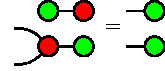
\includegraphics{equation_copy}
				\caption{Copy equation}
			\end{subfigure}%
			~
			\begin{subfigure}[t]{0.3\textwidth}
				\centering
				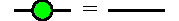
\includegraphics{equation_trivial_spider}
				\caption{Trivial spider equation}
			\end{subfigure}%
			%%%%%%%%%%%%%%%%%%%%%%
			\vspace{2ex}
			%%%%%%%%%%%%%%%%%%%%%%
			\begin{subfigure}[t]{0.33\textwidth}
				\centering
				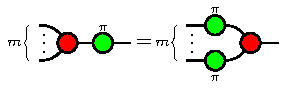
\includegraphics{equation_pi_copy}
				\caption{$\pi$-Copy equation}
			\end{subfigure}%
			~
			\begin{subfigure}[t]{0.33\textwidth}
				\centering
				
\includegraphics{equation_pi_commutation}
				\caption{$\pi$-Commutation equation}
			\end{subfigure}%
			~
			\begin{subfigure}[t]{0.33\textwidth}
				\centering
				
\includegraphics{equation_loop}
				\caption{Loop equation}
			\end{subfigure}%
			%%%%%%%%%%%%%%%%%%%%%%
			\vspace{2ex}
			%%%%%%%%%%%%%%%%%%%%%%
			\begin{subfigure}[t]{0.4\textwidth}
				\centering
				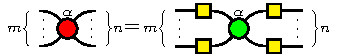
\includegraphics{equation_color_change}
				\caption{Color change equation}
			\end{subfigure}%
			~
			\begin{subfigure}[t]{0.4\textwidth}
				\centering
				
\includegraphics{equation_diamond}
				\caption{Diamond equation}
			\end{subfigure}%
			%%%%%%%%%%%%%%%%%%%%%%
		\end{minipage}
	}
	\caption{Relations in the category $\cat{zx}$}
	\label{fig:ZX equations}
\end{figure}

Thus far, we have a presentation for a free dagger compact category. However, there are relations that between $\cat{zx}$-morphisms.  The emergence of these relations is technical and the interested reader should read about the genesis of the zx-calculus \cite{CoeckeDuncan_QuantumObsFullPaper} to learn the story. To the generating relations of $\cat{zx}$ depicted in Figure \ref{fig:ZX equations}, we add equations obtained by exchanging red and green nodes, daggering, and taking the diagrams up to ambient isotopy in $4$-space. These listed relations will be called \emph{basic}. Note that we denote the empty graph, which is the monoidal unit, by $\emptyset$. Also, spiders with no phase indicated have a phase of $0$. 

A major advantage of using these string diagrams, besides their intuitive nature, is that computations are more easily encoded into computer programs.  Indeed, software programs such as Quantomatic \cite{BarKissingerVicary_Globular,DixonDuncanKissinger_QuantomaticWebsite} and Globular \cite{BarKissingerVicary_Globular} are graphical proof assistants tailor made for such graphical reasoning.  The logic of these programs are encapsulated by double pushout rewrite rules.  However, the algebraic structure of $\cat{zx}$ and other graphical calculi do not contain the rewrite rules as explicit elements.  It is the author's hope that introducing rewrite rules into the algebraic structures embodying graphical calculi, a positive contribution will be made to these programs.  

%%%%%%%%%%%%%%%%%%%%%%
%%%%%%%%%%%%%%%%%%%%%%
% A BICATEGY FOR REWRITING OPEN GRAPHS
\section{Rewriting open graphs}
\label{sec:RewritingOpenGraphs}
%%%%%%%%%%%%%%%%%%%%%%
%%%%%%%%%%%%%%%%%%%%%%

Now that we have seen depictions of the $\cat{zx}$-morphisms, it is clear that they are reminiscent of directed graphs.  There is reason to be optimistic that graphs can model the zx-calculus using graphs.  However, our hope is tempered by the fact that there are clear differences between graphs and $\cat{zx}$-morphisms.  For instance, graphs do not have inputs or outputs. In this section, we reconcile this particular difference by presenting the notion of an open graph.

Intuitively, the notion of an open graph is rather simple.  Take a directed graph and declare some of the nodes to be inputs and others to be outputs, for instance
\[
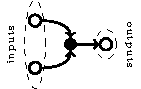
\includegraphics{example_open_graph_1}
\]
Whenever there is a bijection between the inputs of one graph and the outputs of another, we can identify them as described by the bijection.  This process is provides a way to turn a pair of compatible open graphs into a single open graph.  For instance, to the above open graph, we can connect 
\[
	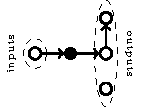
\includegraphics{example_open_graph_3}
\]
to form the open graph
\[
	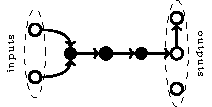
\includegraphics{example_open_graph_4}
\]
This is made precise using cospans and pushout as follows. 

\begin{defn}
\label{def:Open Graph}
	Consider the functor $N \from \cat{Set}_0 \to \cat{Graph}$, on a skeleton of $\cat{Set}$, that is given by the letting $N(X)$ be the edgeless graph with nodes $X$.  An \emph{open graph} is then a cospan in the category $\cat{Graph}$ of the form $N(X) \to G \gets N(Y)$ for sets $X$ and $Y$.
\end{defn}

The left leg $N(X)$ of the cospan are the \emph{inputs} and the right leg $N(Y)$ are the \emph{outputs}.  Suppose we have another open graph $G'$ with inputs $N(Y)$ and outputs $N(Z)$.  Then we can compose cospans 
\[
N(X) \to G \gets N(Y) \to G' \gets N(Z). 
\] 
by pushing out over $G \gets N(Y) \to G'$ to get 
\[
N(X) \to G +_{N(Y)} G' \gets N(Z).
\] 
By taking isomorphism classes of these pushouts, we obtain a category whose objects are those in the image of $N$ and morphisms are open graphs. But we can do better! 

Thus far, we have only just described the first layer of a symmetric monoidal and compact closed (SMCC) bicategory named $\cat{Rewrite'}$.  This bicategory was introduced by the author, though without the prime \cite{Cicala_SpansCospans}. It was shown that $\cat{Rewrite'}$ is SMCC in a joint work with Courser \cite{CicalaCourser_BicatSpansCospan}. The monoidal structure is induced from the coproduct of graphs.  However, for our purposes, there are technical reasons to make a slight adjustment to $\cat{Rewrite'}$.  To create our revised version, $\cat{Rewrite}$, we begin by defining a new bicategory.

Given a category $\cat{C}$, we can talk about spans of cospans in $\cat{C}$.  They and their morphisms are simply commuting diagrams of a certain shape illustrated in Figure \ref{fig:spans of cospans}.  We are interested in morphism classes of spans of cospans, by which we mean the equivalence relation generated on the spans of cospans by relating $S$ and $S'$ if there is a morphism of spans of cospans $S \to S'$.  One can alternatively conceive a morphism class as an isomorphism class of spans of cospans in the image of the inclusion functor $\cat{C} \hookrightarrow \widehat{\cat{C}}$ where $\widehat{\cat{C}}$ is the groupoid generated by $\cat{C}$.   

\begin{thm}
\label{thm:SpCspC is SMCC bicategory}
	If $\cat{C}$ has finite limits and colimits, there is an SMCC bicategory $\bispcs{C}$ consisting of objects of $\cat{C}$ as $0$-cells, cospans in $\cat{C}$ as $1$-cells, and morphism classes of spans of cospans in $\cat{C}$ as $2$-cells. 
\end{thm}
\begin{proof}
	By appropriately modifying the authors work in \cite{Cicala_SpansCospans}, one can show that $\bispcs{C}$ is a bicategory.  A slight change in arguments found in the authors joint work with Courser \cite{CicalaCourser_BicatSpansCospan}, we get that $\bispcs{C}$ is symmetric monoidal and compact closed.
\end{proof}

Showing that $\bispcs{C}$ is symmetric monoidal relied heavily on Shulman's technique involving symmetric monoidal double categories \cite{Shulman_ConstructSMBicats}. The monoidal product is induced by the coproduct on $\cat{C}$.

Recall that  $2$-cells can be composed in two ways in a bicatgory.  Horizontal composition in $\bispcs{C}$ uses pushouts and vertical composition uses pullbacks, as illustrated here:
\begin{equation}
\label{eq:Hor and Vert Composition}
	\raisebox{-0.85\height}{%
	\raisebox{0.3\height}{%
		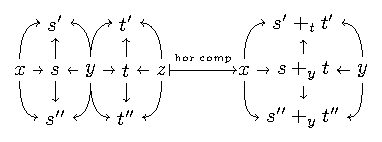
\includegraphics[scale=0.85]{scC_horizontal_composition} 
	}
	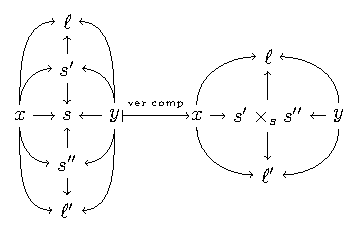
\includegraphics[scale=0.85]{scC_vertical_composition}
}
\end{equation}

\begin{defn}
	Define $\cat{Rewrite}$ to be the $1$-full and $2$-full SMCC sub-bicategory of $\bispcs{Graph}$ whose  $0$-cells are exactly graphs in the image of the functor $N \from \cat{Set}_0 \to \cat{Graph}$.
\end{defn}

The concept of $\cat{Rewrite}$ is that the $1$-cells are open graphs and the $2$-cells are rewrite rules that preserves the input and output nodes. By rewrite rules, we mean those taken from the double pushout graph rewriting approach \cite{Corradini_AlgAppGraphTrans}. 

Our motivation for constructing $\cat{Rewrite}$ is not necessarily to study it directly, but rather for it to serve as an ambient context in which to generate SMCC sub-bicategories on some collection of open graphs and rewriting rules. This is worth considering because many graphical calculi use some version of open graphs as a semantics and with equations between graphical terms given by rewrite rules \cite{Dixon_OpenGraphs,Fong_AlgOpenSystems,Pollard_OpenMarkov}.   There are drawbacks to this approach. For example, working with open graphs is only useful to model graphical calculi whose terms are equal up to ambient isotopy in $4$-space. This limits the current approach to only symmetric monoidal (bi)categories as Selinger's shows in his work \cite{Selinger_GraphicsMonCats} excellently describing various graphical calculi and the role ambient isotopy plays in their use. 

%%%%%%%%%%%%%%%%%%%%%%
%%%%%%%%%%%%%%%%%%%%%%
% OPEN STRUCTURED GRAPHS
\section{Open graphs over $S\zx$}
\label{sec:OpenGraphsOverSzx}
%%%%%%%%%%%%%%%%%%%%%%
%%%%%%%%%%%%%%%%%%%%%%

So far, in Section \ref{sec:RewritingOpenGraphs}, we saw that there is an SMCC bicategory $\bispcs{C}$. In particular, we discussed its sub-bicategory $\cat{Rewrite}$.  While, the $\cat{zx}$-morphisms are like open graphs with multi-sorted nodes, $\cat{Rewrite}$ is not good enough for our purposes. It can capture the openness, but is not strong enough to see the multi-sortedness of the node.  We need some new construction, analogous to $\cat{Rewrite}$, with this additional structure. In this section, we determine exactly what structure is needed and produce the desired SMCC bicategory, $\cat{zxRewrite}$. 

\begin{defn}
	
Let $S$ be a graph.  By a \emph{graph over $S$}, we mean a graph morphism $G \to S$. A morphism between graphs over $S$ is a graph morphism $G \to G'$ such that 
\[
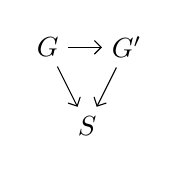
\begin{tikzpicture}
\node (1) at (-0.5,1) {$G$};
\node (2) at (0.5,1) {$G'$};
\node (3) at (0,0) {$S$};
%
\path[->,font=\scriptsize,>=angle 90]
(1) edge (2)
(1) edge (3)
(2) edge (3);
\end{tikzpicture}
\]
commutes.
\end{defn} 

Using graphs over $S$, for a particular $S$, will provide the multi-sorted nodes we seek. Essentially,  $G$ absorbs the structure of $S$ via the fibres of the morphism. We illustrate this with the following example.

\begin{ex}
\label{ex:basic graph over Szx}
	Let $S_{\text{zx}}$ be the graph
\begin{equation}
\label{diag:zx struture graph}
\raisebox{-0.75\height}{
	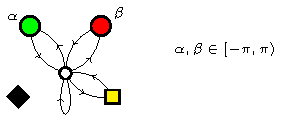
\includegraphics{graph_S_zx}
}
\end{equation}

We have not drawn the entirety of $S_{\text{zx}}$. In actuality, the green and red nodes run through $[-\pi,\pi)$ and all of them have a single arrow to and from node 
$

\begin{tikzpicture}
	\node [zxopen] at (0,0) {};
\end{tikzpicture}
$. 

Most of the structure of the basic $\cat{zx}$-morphisms is captured by graphs over $S_{\text{zx}}$:
\[
	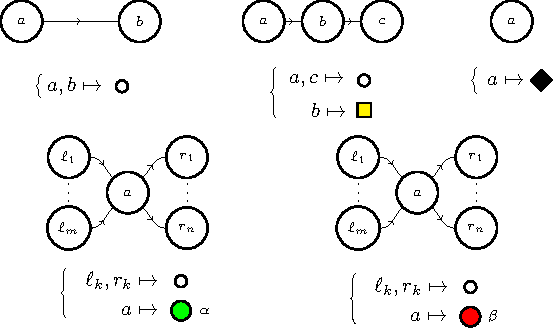
\includegraphics[scale=0.9]{graph_over_Szx}
\]
Note that the functions are completely determined by their behavior on the nodes because there is at most one arrow between any two nodes in $S_{\text{zx}}$.  The role each of the nodes in $S_{\text{zx}}$ plays in providing structure is evident except, perhaps, for the node
$

\begin{tikzpicture}
\node [zxopen] at (0,0) {};
\end{tikzpicture}
$.   
Observe that four of the basic $\cat{zx}$-morphisms have dangling wires on either end.  Because edges of directed graphs must be attached to a pair of nodes, we use this node to anchor the dangling edges.
\end{ex}

\begin{ex}
\label{ex:graph over Szx}
At this point, we can think of the basic elements of the zx-calculus as graphs over $S_{\text{zx}}$. But we can actually do this for any $\cat{zx}$-morphism, such as
\[
	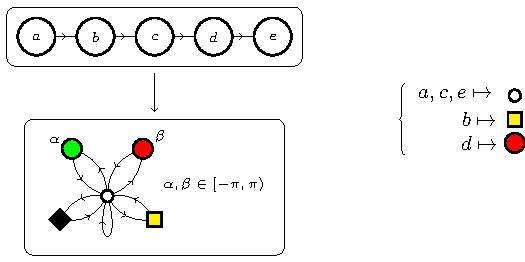
\includegraphics[scale=0.9]{example_graph_over_Szx}
\]
This corresponds with the $\cat{zx}$-morphism 
\[
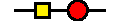
\includegraphics{example_zx_morphism_as_graph_over_Szx}
\]
\end{ex}

Above, we mentioned that the graphs over $S\zx$ from Example \ref{ex:basic graph over Szx} capture `most' of the structure of the basic $\cat{zx}$-morphisms.  The difference is, basic $\cat{zx}$-morphisms are composable. Therefore, if we aim to describe $\cat{zx}$-morphisms with graphs over $S\zx$, we need to be able to connect graphs over $S_{\text{zx}}$ in a way that captures composition. We can achieve this by equipping graphs over $S_{\text{zx}}$ with inputs and outputs, just as we did for open graphs.  Again, we use cospans, though the added structure introduces new considerations. 

Consider the over category $\zxGraphs$ of graphs over $S_{\text{zx}}$. By Theorem \ref{thm:SpCspC is SMCC bicategory}, this gives us an SMCC bicategory $\cat{Sp}(\cat{Csp}(\cat{Graph}\downarrow S_{\text{zx}}))$  within which we would like to construct a sub-bicategory in a similar vein to $\cat{Rewrite}$.  However, there is a problem.  Recall that the objects of $\cat{Rewrite}$ have the form $N(X)$ where $N \from \cat{Set}_0 \to \cat{Graph}$ is the functor sending a set to the edgeless graph on that set.  In $\cat{Graph}$, there is a unique way to be an edgeless graph. But in $\zxGraphs$, there is no unique way to be edgeless because there may be more than one graph morphism to $S_{\text{zx}}$. For instance, the graph with two nodes and no edges can be a graph over $S_{\text{zx}}$ in $5^2 = 25$ ways. This issue can be rectified by functorially choosing which edgeless graphs over $S_{\text{zx}}$ will serve as inputs and outputs. 

\begin{defn}
\label{def:Nzx functor}
	Define a functor 
	\[
		N_{\text{zx}} \from \cat{Set}_0 \to \zxGraphs
	\] 
	by $X \mapsto (N_{\text{zx}}(X) \to S_{\text{zx}})$ where $N_{\text{zx}}(X)$ is the edgeless graph with nodes $X$ that are constant over $
\begin{tikzpicture} \node [zxopen] at (0,0) {}; \end{tikzpicture}$. An \emph{open graph over $S_{\text{zx}}$} is a cospan in $\zxGraphs$ of the form
	\[
		N_{\text{zx}}(X) \to G \gets N_{\text{zx}} (Y).
	\]
\end{defn}

With $N\zx$ in hand, we can expand the notion of graphs over $S\zx$ to open graphs over $S\zx$.  At this point, we are ready to define the analogue to $\cat{Rewrite}$. 

\begin{defn}
	Define a bicategory $\cat{zxRewrite}$ as the symmetric monoidal and compact closed sub-bicategory of $\SpCspZX$ that is $1$-full and $2$-full on the objects of the form $N\zx (X)$ for sets $X$.  
\end{defn}

Unpacking this definition, the $0$-cells of $\cat{zxRewrite}$ are those edgeless graphs over $S\zx$ in the image of $N\zx$.  The $1$-cells are exactly the open graphs over $S\zx$. The $2$-cells are all the ways to rewrite one open graph over $S\zx$ into another in a way that preserves the inputs and outputs.  To better understand this bicategory, we give an example of an open graph over $S_{\text{zx}}$. Along with this example, we introduce new notation in order to keep the remaining diagrams rather compact, which is better illustrated than described.

\begin{ex}
\label{ex:open graph over Szx}
Consider the graph over $S_{\text{zx}}$ in Example \ref{ex:graph over Szx}.  Make this an open graph as follows:
\[
	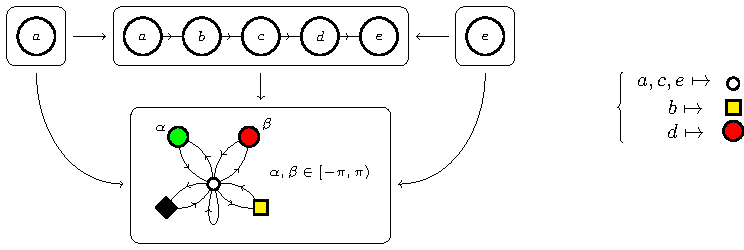
\includegraphics[scale=0.9]{example_open_graph_over_Szx}
\]
There is a single input, node $a$, and a single output, node $e$. Denote this by
\[
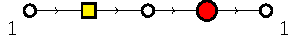
\includegraphics{example_zx_morphism_as_open_graph_over_Szx}
\]
The input nodes are aligned on the far left and the output nodes on the far right.  The $1$'s in the corners refer to the cardinality of the input and output node sets.  This may seem unnecessary or perhaps even redundant, but it will bring clarity to several situations arising later on. Hence, we will side with consistency and write these cardinalities every time.  Also, it is safe to assume that the left and right hand cospan maps are always injections. Even though this is not required by $\cat{zxRewrite}$, it is true throughout this paper.  Of course, this notation sheds away a fair amount information regarding the graph morphisms involved in the cospan, though this information should not be missed.
\end{ex}

As mentioned earlier, our interest in the category $\cat{Rewrite}$ is as an ambient context in which to generate symmetric monoidal and compact closed bicategories from some collection of $1$-cells and $2$-cells. The same can be said for our new bicategory $\cat{zxRewrite}$.  Presently, we are interested in $1$-cells that correspond to the basic $\cat{zx}$-morphisms from Figure \ref{fig:ZX generators} and $2$-cells that correspond to the basic relations from Figure \ref{fig:ZX equations}.  Our claim is that the bicategory generated by these $1$-cells and $2$-cells categorifies $\cat{zx}$.

%%%%%%%%%%%%%%%%%%%%%%
%%%%%%%%%%%%%%%%%%%%%%
% ZX CATEGORIFIED
\section{A categorification of $\cat{zx}$}
\label{sec:zx categorified}
%%%%%%%%%%%%%%%%%%%%%%
%%%%%%%%%%%%%%%%%%%%%%

The basic $\cat{zx}$-morphisms in Figure \ref{fig:ZX generators} are naturally presented as open graphs over $S_{\text{zx}}$ as shown in Figure \ref{fig:ZX 1cells generators}.  We will refer to these five diagrams as \emph{basic}.  To clarify the double instances of $m$ and $n$ written in the spider diagrams, those written on the bottom of the diagram refer to the cardinalities of the cospan legs, and those written beside the brackets count how many nodes are there.  The injectivity of the cospan legs of these generators ensure that these numbers will be the same for the basic diagrams.

\begin{figure}[h]
	\fbox{%
		\begin{minipage}{\textwidth}
			\centering
			%%%%%%%%%%%%%%%%%%%%%%
			\subcaptionbox{Wire}[.30\textwidth]{%
				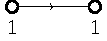
\includegraphics{1cell_zx_wire}
			}
			~
			\subcaptionbox{Hadamard}[.30\textwidth]{%
				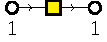
\includegraphics[]{1cell_zx_hadamard}
			}
			~
			\subcaptionbox{Diamond}[.30\textwidth]{%
				
\includegraphics{1cell_zx_diamond}
			}
			\linebreak
			\subcaptionbox{Green spider}[.4\textwidth]{%
				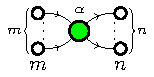
\includegraphics{1cell_zx_green_spider}
			}
			~
			\subcaptionbox{Red spider}[.4\textwidth]{%
				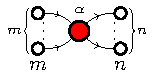
\includegraphics{1cell_zx_red_spider}
			}
			%%%%%%%%%%%%%%%%%%%%%%
		\end{minipage}
	}
	\caption{Generating $1$-cells for the bicategory $\bicat{zx}$}
	\label{fig:ZX 1cells generators}
\end{figure} 

Just as the open graphs over $S_{\text{zx}}$ in Figure \ref{fig:ZX 1cells generators} capture the generating $\cat{zx}$-morphisms, we also want to introduce the basic relations into our framework.  These relations are presented in Figure \ref{fig:ZX 2cells generators}, but we also include $2$-cells obtained by exchanging red and green nodes, swapping inputs and outputs for each graph over $S\zx$, or by turning the spans around.  There is also an additional $2$-cell
\[
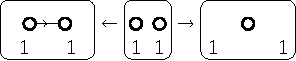
\includegraphics{2cell_wire_is_identity}
\]
added to account for the fact that the wire $1$-cell is not the identity on $1$ here. This $2$-cell will allow us to replace a wire with an identity. All of these $2$-cells, we call \emph{basic}.  We are now ready to define the bicategory which categorifies the zx-calculus.

\begin{figure}[h]
	\fbox{%
		\begin{minipage}{\textwidth}
			\centering
			%%%%%%%%%%%%%%%%%%%%%%
			\subcaptionbox{Spider}[\textwidth]{%
				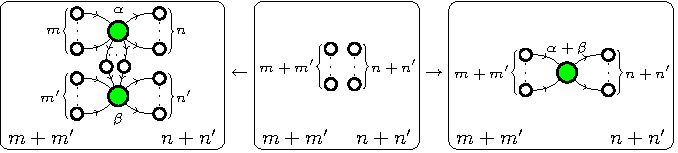
\includegraphics[scale=0.75]{2cell_spider}
			}
			\linebreak
			\subcaptionbox{Bialgebra}[\textwidth]{%
				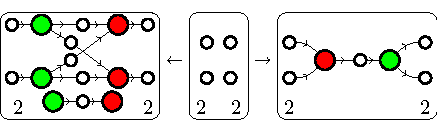
\includegraphics[scale=0.75]{2cell_bialgebra}
			}
			\linebreak
			\subcaptionbox{Cup}[0.45\textwidth]{%
				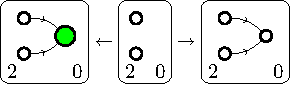
\includegraphics[scale=0.75]{2cell_cup}
			}
			\subcaptionbox{Copy}[0.45\textwidth]{%
				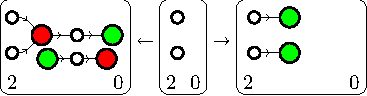
\includegraphics[scale=0.75]{2cell_copy}
			}
			\linebreak
			\subcaptionbox{Trivial spider}[0.45\textwidth]{%
				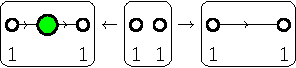
\includegraphics[scale=0.75]{2cell_trivial_spider}
			}
			\subcaptionbox{$\pi$-copy}[0.45\textwidth]{%
				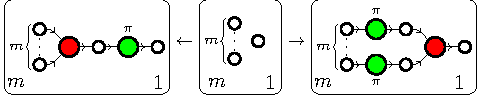
\includegraphics[scale=0.75]{2cell_pi_copy}
			}
			\linebreak
			\subcaptionbox{$\pi$-commutation}[\textwidth]{%
				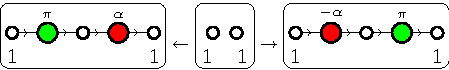
\includegraphics[scale=0.75]{2cell_pi_commutation}
			}
			\linebreak
			\subcaptionbox{Color change}[\textwidth]{%
				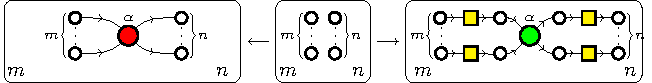
\includegraphics[scale=0.75]{2cell_color_change}
			}
			\linebreak
			\subcaptionbox{Loop}[0.45\textwidth]{%
				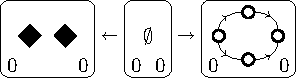
\includegraphics[scale=0.75]{2cell_loop}
			}
			\subcaptionbox{Diamond}[0.45\textwidth]{%
				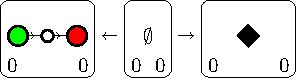
\includegraphics[scale=0.75]{2cell_diamond}
			}
			%%%%%%%%%%%%%%%%%%%%%%
		\end{minipage}
	}
	\caption{Generating $2$-cells for the bicategory $\bicat{zx}$}
	\label{fig:ZX 2cells generators}
\end{figure}

\begin{defn}
	\label{def:zx bicat}
	Define $\bicat{zx}$ to be the symmetric monoidal and compact closed sub-bicategory of $\cat{zxRewrite}$ generated by the basic $1$-cells and basic $2$-cells.
\end{defn}

Because $\bicat{zx}$ is symmetric monoidal and compact closed, it also contains a twist $1$-cell, plus evaluation and coevaluation $1$-cells for the compact structure on $m$ 
\begin{equation}
\label{diag:TwistCompact 1cells}
\raisebox{-0.8\height}{
	\includegraphics[scale=0.75]{1cell_zx_braiding}
	\quad \quad \quad
	\includegraphics[scale=0.75]{1cell_zx_evaluation}
	\quad \quad \quad
	\includegraphics[scale=0.75]{1cell_zx_coevaluation}
}
\end{equation}
Horizontal and vertical composition acts just as in \eqref{eq:Hor and Vert Composition}. For example, we can compose spider diagrams with the same number of inputs and outputs:
\[
	\includegraphics{example_composing_spiders}
\]
Tensoring $1$-cells is simply disjoint union: 
\[
	\includegraphics{diagram_tensor_spiders}
\]
Having defined $\bicat{zx}$, we can turn our focus towards presenting the main theorem. We start with the following definition.

\begin{defn}
\label{def:decat zx}
	Define $\decat(\bicat{zx})$ to be the category whose objects are the $0$-cells of $\bicat{zx}$ and whose arrows the $1$-cells of $\bicat{zx}$ modulo the equivalence relation $\sim$ given by: $f \sim g$ if and only if there is a $2$-cell $f \Rightarrow g$ in $\bicat{zx}$.
\end{defn}

To be clear, the above actually is an equivalence relation and doesn't merely generate one.  This follows from the symmetry of spans and vertical composition.   

\begin{thm}
\label{thm:decat zx is dagger compact}
	The category $\decat(\bicat{zx})$ is dagger compact via the identity on objects functor described by 
	\[
	\raisebox{-0.5\height}{%
	\includegraphics{functor_dagger_decat_zx_spider_green}
	}
	\quad \text{and} \quad
	\raisebox{-0.5\height}{%
	\includegraphics{functor_dagger_decat_zx_spider_red}
	}
	\]
	as well as by identity on the wire, Hadamard, and diamond morphisms.
\end{thm}
\begin{proof}
	Compact closedness follows from the self duality of objects via the evaluation and coevaluation maps from \eqref{diag:TwistCompact 1cells}. Moreover, we can derive the snake equation
	\[
		\includegraphics[scale=0.75]{equation_decat_zx_snake}
	\]
	where the equalities follow from the evident $2$-cells in $\bicat{zx}$. The extra relation introduced in Definition \ref{def:zx bicat} ensures that the string of wires is the identity.  Showing that the described functor is a dagger functor is a matter of checking some easy to verify details. 
\end{proof}

\begin{thm}
\label{thm:equiv of zx cats}
	The identity on objects, dagger compact functor $E \from \cat{zx} \to \decat(\bicat{zx})$ given by
	\begin{center}
	\begin{tabular}{lr}
		$
		\raisebox{-0.4\height}{\includegraphics{generater_green_spider} }
		\mapsto
		\raisebox{-0.55\height}{\includegraphics{1cell_zx_green_spider}}
		$
		&
		$
		\raisebox{-0.45\height}{\includegraphics{generater_wire}}
		\mapsto
		\raisebox{-0.65\height}{\includegraphics{1cell_zx_wire}}
		$
	\end{tabular}

	\begin{tabular}{lcr}
		$
		\raisebox{-0.35\height}{\includegraphics{generater_red_spider}}
		\mapsto
		\raisebox{-0.55\height}{\includegraphics{1cell_zx_red_spider}}
		$
		&
		$
		\raisebox{-0.3\height}{\includegraphics{generater_diamond}}
		\mapsto
		\raisebox{-0.65\height}{\includegraphics{1cell_zx_diamond}}
		$
		&
		$
		\raisebox{-0.2\height}{\includegraphics{generater_hadamard}}
		 \mapsto
		\raisebox{-0.65\height}{\includegraphics{1cell_zx_hadamard}}
		$
	\end{tabular}
	\end{center}
	is an equivalence of categories.
\end{thm}
\begin{proof}
	Essential surjectivity follows immediately from $E$ being identity on objects.  Fullness follows from the fact that the morphism generators for $\decat(\bicat{zx})$ are all in the image of $E$. 
	
	Faithfulness is more involved. Let $f,g$ be $\cat{zx}$-morphisms. Let $\widetilde{Ef}$, $\widetilde{Eg}$ be the representatives of $Ef$, $Eg$ obtained by directly translating the graphical representation of $f,g$ to open graphs of $S\zx$ as in Examples \ref{ex:graph over Szx}  and \ref{ex:open graph over Szx}. For faithfulness, it suffices to show that the existence of a $2$-cell $\widetilde{Ef} \Rightarrow \widetilde{Eg}$ in $\bicat{zx}$ implies that $f=g$.  
	
	Observe that any $2$-cell $\alpha$ in $\bicat{zx}$ can be written, not necessarily uniquely, as sequence $\alpha_1 \square \dotsm \square \alpha_n$ of length $n$ where each $\alpha_i$ is a basic $2$-cell and each box is filled in with `$\circ_\t{h}$', `$\circ_\t{v}$', or `$+$'. By `$\circ_\t{h}$' and `$\circ_\t{v}$', we mean horizontal and vertical composition. We will induct on sequence length.  If $\alpha \from \widetilde{Ef} \Rightarrow \widetilde{Eg}$ is a basic $2$-cell, then there is clearly a corresponding basic relation equating $f$ and $g$.  Suppose we have a sequence of length $n+1$ such that the left-most square is a `$+$'. Rhen we have a $2$-cell $\alpha_1 + \alpha_2 \from Ef \Rightarrow Eg$ where $\alpha_1$ is a basic $2$-cell and $\alpha_2$ can be written with length $n$.   By fullness, we can write $\alpha_1 + \alpha_2 \from Ef_1 + EF_2 \Rightarrow Eg_1 + Eg_2$ where $\alpha_i \from Ef_i \Rightarrow Eg_i$.   This gives that $f_i = g_i$  and the result follows.  A similar argument handles the cases when the left-most operation is vertical or horizontal composition.
\end{proof}

%%%%%%%%%%%%%%%%%%%%%%%%%%%%%%%%%%%%%%%
%%%%%%%%%%%%%%%%%%%%%%%%%%%%%%%%%%%%%%%
%
% BIBLIOGRAPHY
%
%%%%%%%%%%%%%%%%%%%%%%%%%%%%%%%%%%%%%%%
%%%%%%%%%%%%%%%%%%%%%%%%%%%%%%%%%%%%%%%

\begin{thebibliography}{100}	
	%
	\bibitem{AbramCoecke_CatSemanticQuantum}
	S.~Abramsky \& B.~Coecke
	(2004)
	\emph{A categorical semantics of quantum protocols}. 
	In Logic in Computer Science. 
	Proceedings of the 19th Annual IEEE Symposium on (pp. 415-425). 
	IEEE.
	Chicago.
	Also available as \href{https://arxiv.org/abs/quant-ph/0402130}{	arXiv:quant-ph/0402130}.
	%
	\bibitem{Backens_Completeness}
	M.~Backens
	(2016)
	\emph{Completeness and the ZX-calculus.} 
	Available as \href{https://arxiv.org/abs/1602.08954}{arXiv:1602.08954}.
	%
	\bibitem{BaezFongPollard_CompMarkovProcesses}
	J.~Baez, B.~Fong, \& B.~Pollard
	(2016)
	\emph{A compositional framework for Markov processes}. 
	Journal of Mathematical Physics, 
	57(3), 033301.
	Also available as \href{https://arxiv.org/abs/1508.06448}{arXiv:1508.06448}.
	%
	\bibitem{BarKissingerVicary_Globular}
	K.~Bar, A.~Kissinger, \& J.~Vicary
	(2016)
	\emph{Globular: an online proof assistant for higher-dimensional rewriting}. 
	1st International Conference on Formal Structures for Computation and Deduction,
	vol. 52, pp.~1–11.
	\href{http://globular.science}{http://globular.science}
	%
	\bibitem{Cicala_SpansCospans} 
	D.~Cicala
	(2016)
	\emph{Spans of cospans}.
	Available as \href{https://arxiv.org/abs/1611.07886}{arXiv:1611.07886}.
	%
	\bibitem{CicalaCourser_BicatSpansCospan}
	D.~Cicala \& K.~Courser,
	\emph{Bicategories of spans and cospans}.
	In preparation.
	%
	\bibitem{CoeckeDuncan_QuantumObsInitialReport}
	B.~Coecke \& R.~Duncan 
	(2008) 
	\emph{Interacting Quantum Observables}. 
	In: Aceto L., Damgård I., Goldberg L.A., Halldórsson M.M., Ingólfsdóttir A., Walukiewicz I. (eds) 
	Automata, Languages and Programming. 
	ICALP 2008. 
	Lecture Notes in Computer Science, vol 5126. 
	Springer, Berlin, Heidelberg
	%
	\bibitem{CoeckeDuncan_QuantumObsFullPaper}
	B.~Coecke \& R.~Duncan
	(2011)
	\emph{Interacting quantum observables: categorical algebra and diagrammatics}. 
	New Journal of Physics, 13(4), 043016.
	Also available as \href{https://arxiv.org/abs/0906.4725}{arXiv:0906.4725}.
	%
	\bibitem{CoeckeEdwards_ToyTheories}
	B.~Coecke \& B.~Edwards
	(2011)
	\emph{Toy quantum categories}.
	In: Proceedings of Quantum Physics and Logic/Development of Computational Models (QPL-DCM).
	Electronic Notes in Theoretical Computer Science,
	271(1), pp.~29-40.
	Also available as \href{https://arxiv.org/abs/0808.1037}{arXiv:0808.1037}.
	%
	\bibitem{CoeckeEdwardsSpekkens_PhaseGrpsNonLocality}
	B.~Coecke, B.~Edwards, \& R.~Spekkens
	(2011)
	\emph{Phase groups and the origin of non-locality for qubits}.
	Electronic Notes in Theoretical Computer Science,
	271(2), pp.~15-36.
	Also available as \href{https://arxiv.org/abs/1003.5005}{arXiv:1003.5005}.
	%
	\bibitem{CoeckePavlovic_QuantumMeasSums}
	B.~Coecke \& D.~Pavlovic
	(2006)
	\emph{Quantum measurements without sums}. 
	Available as \href{https://arxiv.org/abs/quant-ph/0608035}{arXiv:quant-ph/0608035}.
	%
	\bibitem{CoeckePavVicary_OrthBasis}
	B.~Coecke, D.~Pavlovic, \& J.~Vicary
	(2013)
	\emph{A new description of orthogonal bases}. 
	Mathematical Structures in Computer Science, 23(03), pp.~555-567.
	Also available as \href{https://arxiv.org/abs/0810.0812}{arXiv:0810.0812}.
	%
	\bibitem{CoeckePerdix_EnvironClassicChannels}
	B.~Coecke \& S.~Pedrix
	(2010)
	\emph{Environment and classical channels in categorical quantum mechanics}.
	In: Proceedings of the 19th EACSL Annual Conference on Computer Science Logic (CSL),
	Lecture Notes in Computer Science 6247, pp.~230-244,
	Springer-Verlag.
	Also available as \href{https://arxiv.org/abs/1004.1598}{arXiv:1004.1598}
	%
	\bibitem{Corradini_AlgAppGraphTrans}
	A.~Corradini, U.~Montanari, F.~Rossi, H.~Ehrig, R.~Heckel, \& M.~L\"{o}we
	(1997).
	\emph{Algebraic Approaches to Graph Transformation-Part I: Basic Concepts and Double Pushout Approach}. 
	In Handbook of Graph Grammars, pp.~163-246.
	%
	\bibitem{DanosKashefiPanang_MeasurementCalc}
	V.~Danos, E.~Kashefi, \& P.~Panangaden,
	(2007)
	\emph{The measurement calculus}. 
	Journal of the ACM (JACM), 54(2), 8.
	Also available as \href{https://arxiv.org/abs/0704.1263}{arXiv:0704.1263}
	%
	\bibitem{Dixon_OpenGraphs}
	L.~Dixon, R.~Duncan, \& A.~Kissinger
	(2010)
	\emph{Open graphs and computational reasoning}. 
	Available as \href{https://arxiv.org/abs/1007.3794}{arXiv:1007.3794}.
	%
	\bibitem{DixonDuncanKissinger_QuantomaticWebsite}
	L.~Dixon, R.~Duncan, \& A.~Kissinger
	\emph{Quantomatic}. \\
	\href{https://sites.google.com/site/quantomatic/}{https://sites.google.com/site/quantomatic/}
	%
	\bibitem{DuncanPerdix_GraphStatesEulerDecomp}
	R.~Duncan \& S.~Perdrix 
	(2009) 
	\emph{Graph States and the Necessity of Euler Decomposition}. 
	In: Ambos-Spies K., Löwe B., Merkle W. (eds) 
	Mathematical Theory and Computational Practice. 
	CiE 2009. 
	Lecture Notes in Computer Science, vol 5635. 
	Springer, Berlin, Heidelberg.
	%
	\bibitem{DuncanPerdrix_RewritingQuantumCompu}
	R.~Duncan, \& S.~Perdrix
	(2010)
	In: Abramsky S., Gavoille C., Kirchner C., Meyer auf der Heide F., Spirakis P.G. (eds)
	\emph{Rewriting measurement-based quantum computations with generalised flow}. 
	ICALP 2010. 
	Lecture Notes in Computer Science, vol 6199. 
	Springer, Berlin, Heidelberg.
	%
	\bibitem{EvansDuncanLangPanan_ClassMutualUnbias}
	J.~Evans, R.~Duncan, A.~Lang, \& P.~Panangaden
	(2009)
	\emph{Classifying all mutually unbiased bases in Rel}.
	Available as \href{https://arxiv.org/abs/0909.4453}{arXiv:0909.4453}
	%
	\bibitem{Fong_AlgOpenSystems}
	B.~Fong
	(2016)
	\emph{The Algebra of Open and Interconnected Systems}. 
	Available as \href{https://arxiv.org/abs/arXiv:1609.05382}{arXiv:1609.05382}. 
	%
	\bibitem{JoyalStreet_GeomTensorCalc}
	A.~Joyal \& R.~Street
	(1991)
	 \emph{The geometry of tensor calculus, I}. 
	 Advances in Mathematics, 
	 88(1), pp.~55-112.
	 Also available at \\ \href{http://www.sciencedirect.com/science/article/pii/000187089190003P}{http://www.sciencedirect.com/science/article/pii/000187089190003P}.
	%
	\bibitem{KissingerZamd_Quantomatic}
	A.~Kissinger \& V.~Zamdzhiev
	(2015)
	\emph{Quantomatic: A proof assistant for diagrammatic reasoning}. 
	In International Conference on Automated Deduction 
	(pp. 326-336). 
	Springer International Publishing.
	Also available as \href{https://arxiv.org/abs/1503.01034}{arXiv:1503.01034}.
	%
	\bibitem{NielsenChuang_QuantumCompInfo}
	M.~Nielsen \& I.~Chuang
	(2000)
	\emph{Quantum Computation and Quantum Information}.
	Cambridge University Press.
	%
	\bibitem{Pavlovic_QuanClassNondetermCompu}
	D.~Pavlovic
	(2009)
	\emph{Quantum and classical structures in nondeterministic computation}.
	Lecture Notes in Computer Science, 5494, pp.~143-157,
	Springer.
	Also available as \href{https://arxiv.org/abs/0812.2266}{arxiv:0812.2266}
	%
	\bibitem{Penrose_NegDimTensors}
	R.~Penrose
	(1971)
	\emph{Applications of negative dimensional tensors.} 
	Combinatorial mathematics and its applications.  221244.  
	Also available at \href{http://homepages.math.uic.edu/~kauffman/Penrose.pdf}{http://homepages.math.uic.edu/~kauffman/Penrose.pdf}
	%
	\bibitem{Pollard_OpenMarkov}
	B.~Pollard
	(2016)
	\emph{Open Markov processes: A compositional perspective on non-equilibrium steady states in biology}. 
	Entropy, 18(4), pp.~140. 
	Also available as \href{https://arxiv.org/abs/1601.00711}{arXiv:1601.00711}.
	%
	\bibitem{SassoneSobocinski_PetriNets}
	V.~Sassone, \& P.~Soboci\'{n}ski
	(2005)
	\emph{A congruence for Petri nets}. 
	Electronic Notes in Theoretical Computer Science, 
	127(2), pp.~107-120.
	Also available as \href{http://www.sciencedirect.com/science/article/pii/S1571066105001222}{http://www.sciencedirect.com/science/article/pii/S1571066105001222}
	%
	\bibitem{Selinger_GraphicsMonCats}
	P.~Selinger
	(2010)
	\emph{A survey of graphical languages for monoidal categories}. 
	New Structures for Physics, pp. ~289-355. 
	Springer Berlin Heidelberg. 
	Also available as \href{https://arxiv.org/abs/0908.3347}{arXiv:0908.3347}.
	%
	\bibitem{Shulman_ConstructSMBicats} 
	M.~Shulman
	(2010)
	\emph{Constructing symmetric monoidal bicategories}.
	Available as \href{http://arxiv.org/abs/1004.0993}{arXiv:1004.0993}.
	%
	
	

\end{thebibliography}


%%%%%%%%%%%%%%%%%%%%%%%%%%%%%%%%%%%%%%%
%%%%%%%%%%%%%%%%%%%%%%%%%%%%%%%%%%%%%%%
%%%%%%%%%%%%%%%%%%%%%%%%%%%%%%%%%%%%%%%
%
% END DOCUMENT
%
%%%%%%%%%%%%%%%%%%%%%%%%%%%%%%%%%%%%%%%
%%%%%%%%%%%%%%%%%%%%%%%%%%%%%%%%%%%%%%%
%%%%%%%%%%%%%%%%%%%%%%%%%%%%%%%%%%%%%%%
%%%%%%%%%%%%%%%%%%%%%%%%%%%%%%%%%%%%%%%

\end{document}